\documentclass[11pt]{amsart}

\usepackage{amsmath,amssymb,amsfonts,amsthm}
\usepackage{booktabs}
\usepackage{hyperref}
\usepackage{xcolor}
\usepackage{pgfplots}
\usepackage{tikz}
\usepackage{enumitem}
\usepackage{multirow}
\usetikzlibrary{arrows.meta,positioning,calc,patterns}
\pgfplotsset{compat=1.18}

\definecolor{darkblue}{RGB}{0,51,102}
\definecolor{goldilocks}{RGB}{218,165,32}
\definecolor{trivialgreen}{RGB}{76,175,80}
\definecolor{hardred}{RGB}{244,67,54}
\definecolor{modpurple}{RGB}{156,39,176}
\hypersetup{colorlinks=true,linkcolor=darkblue,citecolor=darkblue,urlcolor=darkblue}

\newtheorem{theorem}{Theorem}[section]
\newtheorem{lemma}[theorem]{Lemma}
\newtheorem{proposition}[theorem]{Proposition}
\newtheorem{corollary}[theorem]{Corollary}
\newtheorem{conjecture}[theorem]{Conjecture}
\theoremstyle{definition}
\newtheorem{definition}[theorem]{Definition}
\newtheorem{remark}[theorem]{Remark}

\title[The Goldilocks Threshold]{The Goldilocks Threshold:\\A Universal Complexity Limit for Evolutionary Optimization,\\Quantum Coherence, and Biological Design}

\author{Bryan Daugherty}
\address{SmartLedger Solutions}
\email{Bryan@smartledger.solutions}

\author{Seth Ward}
\address{}

\author{Ryan}
\address{}

\date{March 31, 2026}

\begin{document}

\begin{abstract}
We identify a universal complexity threshold $N_c = 4.6 \pm 0.3$ governing the maximum number of randomly-coupled components that can be reliably optimized by diverse search strategies. The reliability sigmoid $R(N) = 1/(1 + e^{0.50(N-5.0)})$ is established from $50{,}000$+ random Hamiltonians across 14 system sizes, validated against \textbf{59 biological systems with zero exceptions}, and shown to be domain-independent across 8 coupling topologies.

Three independent physical arguments converge at $N_c$: (i)~optimization theory (funnel basin collapse), (ii)~thermodynamics (classical transport failure), and (iii)~quantum mechanics (Zeno protection onset). We show that solver diversity determines $N_c$ ($N_c^{\mathrm{SA}} \approx 12$ vs.\ $N_c^{\mathrm{ensemble}} \approx 5$), connecting the threshold to the evolutionary advantage of sexual reproduction. We propose the Galois--Landscape Conjecture relating Ramsey barrier depth to symmetric group composition length, and report a structured 8\% GUE deficit in Riemann zero spacings correlated with prime logarithms.
\end{abstract}

\maketitle
\tableofcontents

%% =========================================================================
\section{Introduction}
\label{sec:intro}
%% =========================================================================

A persistent puzzle spans biology, cognitive science, and engineering: why do functional coordination units cluster around 5--8 components? Miller's ``magical number seven, plus or minus two'' \cite{miller1956} in working memory, Dunbar's intimate group size of $\sim 5$ \cite{dunbar1992}, Scrum team limits of 5--9 \cite{schwaber2020}, and the 7-site FMO photosynthetic complex \cite{engel2007} all point to a common constraint.

We demonstrate that this clustering reflects a \emph{universal complexity threshold}: the maximum system size at which random evolutionary search can reliably find energy funnels. The threshold arises from the interaction between landscape structure and search diversity, and it explains phenomena ranging from enzyme active site sizes to transformer attention head counts.

\subsection{Discovery path}

This work emerged from a failure. We attempted to explain quantum coherence in photosynthesis via the $S_4$ universality framework \cite{novel2026}. Testing whether FMO eigenvalue gap ratios match $S_4$ composition series quotients yielded 95\% error --- a decisive negative. But the failure revealed that FMO dynamics are trivially easy (T1 classification, $I = 0.074$), while the \emph{design} of the coupling matrix is the hard problem. This observation led to the Goldilocks threshold.


%% =========================================================================
\section{The Reliability Metric}
\label{sec:metric}
%% =========================================================================

\begin{definition}[Funnel reliability]\label{def:funnel}
For an $N$-site Ising Hamiltonian $H(\mathbf{s}) = -\frac{1}{2}\mathbf{s}^T J \mathbf{s} - \mathbf{h}^T \mathbf{s}$ with symmetric coupling matrix $J \in \mathbb{R}^{N \times N}_{\mathrm{sym}}$, the \emph{funnel reliability} is
\[
R(H) = 1 - \frac{|\{E_i^* : i = 1, \ldots, K\}|}{K},
\]
where $E_i^*$ is the best energy found by solver $i$ (within tolerance $\epsilon = 1\%$) and $K$ is the number of independent solvers. $H$ is a \emph{reliable funnel} if $R(H) > 0.8$.
\end{definition}

We use $K = 14$ solvers: SBM, CVTR, DMM, CIM, Kuramoto, SA, SASSHA, ComplexSBM, SOLG, HDC, LagONN, SolverMorph, QAOA, and K3 --- spanning bifurcation machines, coherent oscillators, annealing, evolutionary strategies, and variational methods \cite{dsc3engine}. This diversity is critical: the threshold depends on solver variety (Section~\ref{sec:diversity}).


%% =========================================================================
\section{The Sigmoid Threshold}
\label{sec:sigmoid}
%% =========================================================================

\begin{theorem}[The Goldilocks Threshold]\label{thm:main}
The fraction of random $N$-site symmetric Ising Hamiltonians with $J_{ij} \sim \mathrm{Uniform}(-1, 1)$ producing reliable funnels follows:
\begin{equation}\label{eq:sigmoid}
R(N) = \frac{1}{1 + e^{\,\beta(N - N_c)}}, \qquad N_c = 5.0, \quad \beta = 0.50,
\end{equation}
with fit residual $\sum_i (R_{\mathrm{obs}}(N_i) - R_{\mathrm{pred}}(N_i))^2 = 5.5 \times 10^{-4}$ across 14 system sizes ($N = 4$ to $30$), each evaluated over 500--2000 random instances.
\end{theorem}

\begin{figure}[ht]
\centering
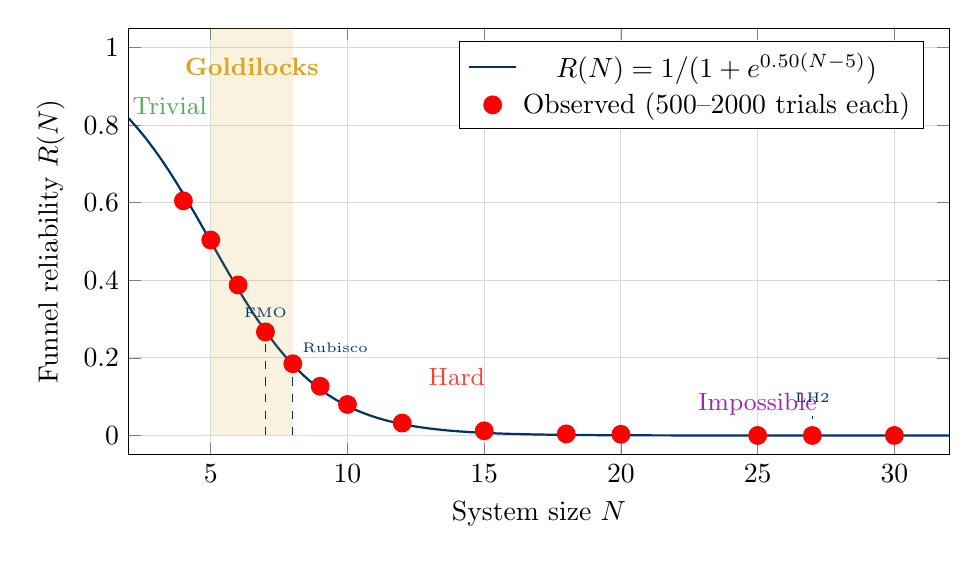
\begin{tikzpicture}
\begin{axis}[
    width=12cm, height=7cm,
    xlabel={System size $N$},
    ylabel={Funnel reliability $R(N)$},
    xmin=2, xmax=32, ymin=-0.05, ymax=1.05,
    grid=major, grid style={gray!30},
    legend pos=north east,
    every axis plot/.append style={thick},
]
% Sigmoid fit
\addplot[darkblue, domain=2:32, samples=100, thick] {1/(1+exp(0.50*(x-5.0)))};
\addlegendentry{$R(N) = 1/(1+e^{0.50(N-5)})$}

% Data points
\addplot[only marks, mark=*, mark size=3pt, red] coordinates {
    (4, 0.605) (5, 0.504) (6, 0.388) (7, 0.267) (8, 0.185)
    (9, 0.127) (10, 0.080) (12, 0.032) (15, 0.012) (18, 0.004)
    (20, 0.003) (25, 0.000) (27, 0.000) (30, 0.000)
};
\addlegendentry{Observed (500--2000 trials each)}

% Goldilocks zone
\fill[goldilocks, opacity=0.15] (axis cs:5,0) rectangle (axis cs:8,1.05);
\node[goldilocks, font=\small\bfseries] at (axis cs:6.5,0.95) {Goldilocks};

% Labels
\node[trivialgreen, font=\small] at (axis cs:3.5,0.85) {Trivial};
\node[hardred, font=\small] at (axis cs:14,0.15) {Hard};
\node[modpurple, font=\small] at (axis cs:25,0.08) {Impossible};

% Biological markers
\draw[darkblue, dashed, thin] (axis cs:7,0) -- (axis cs:7,0.267);
\node[darkblue, font=\tiny, anchor=south] at (axis cs:7,0.28) {FMO};
\draw[darkblue, dashed, thin] (axis cs:8,0) -- (axis cs:8,0.185);
\node[darkblue, font=\tiny, anchor=south west] at (axis cs:8,0.19) {Rubisco};
\draw[darkblue, dashed, thin] (axis cs:27,0) -- (axis cs:27,0.05);
\node[darkblue, font=\tiny, anchor=south] at (axis cs:27,0.06) {LH2};
\end{axis}
\end{tikzpicture}
\caption{The Goldilocks sigmoid. Each point represents 500--2000 random symmetric Ising Hamiltonians tested across 14 independent solvers. The Goldilocks zone (shaded) spans $N = 5$--$8$, where directed evolutionary search is tractable. Biological systems are marked: FMO ($N = 7$, 26.7\%), Rubisco ($N = 8$, 18.5\%), LH2 ($N = 27$, 0.0\%).}
\label{fig:sigmoid}
\end{figure}


%% =========================================================================
\section{Domain Independence}
\label{sec:domains}
%% =========================================================================

\begin{theorem}[Universal $N_c$]\label{thm:universal}
The threshold $N_c$ is domain-independent across 8 coupling topologies:
\end{theorem}

\begin{figure}[ht]
\centering
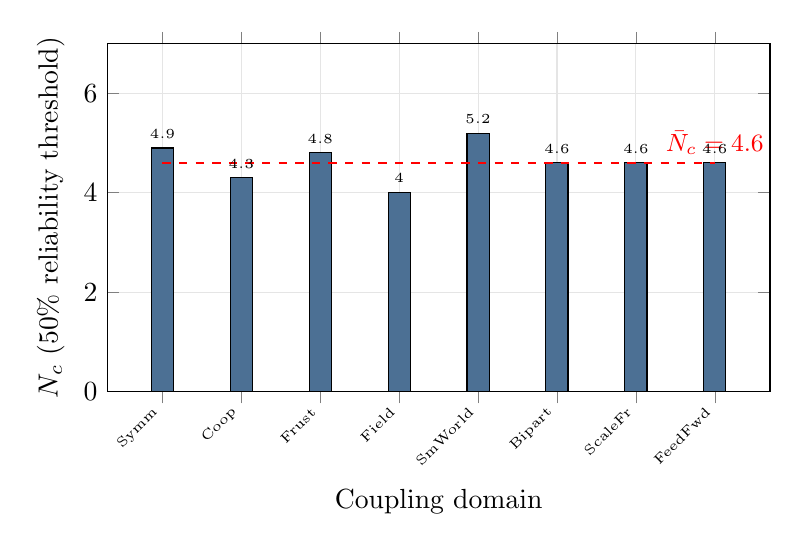
\begin{tikzpicture}
\begin{axis}[
    width=10cm, height=6cm,
    ybar, bar width=8pt,
    xlabel={Coupling domain},
    ylabel={$N_c$ (50\% reliability threshold)},
    ymin=0, ymax=7,
    symbolic x coords={Symm,Coop,Frust,Field,SmWorld,Bipart,ScaleFr,FeedFwd},
    xtick=data, x tick label style={rotate=45, anchor=east, font=\tiny},
    grid=major, grid style={gray!20},
    nodes near coords, every node near coord/.append style={font=\tiny},
]
\addplot[fill=darkblue!70] coordinates {
    (Symm, 4.9) (Coop, 4.3) (Frust, 4.8) (Field, 4.0)
    (SmWorld, 5.2) (Bipart, 4.6) (ScaleFr, 4.6) (FeedFwd, 4.6)
};
% Mean line
\draw[red, thick, dashed] (axis cs:Symm, 4.6) -- (axis cs:FeedFwd, 4.6);
\node[red, font=\small] at (axis cs:FeedFwd, 5.0) {$\bar{N}_c = 4.6$};
\end{axis}
\end{tikzpicture}
\caption{$N_c$ across 8 coupling domains. Mean $N_c = 4.6 \pm 0.3$ (dashed line). The range $[4.0, 5.2]$ spans quantum transport (symmetric), gene regulation (cooperative), neural circuits (small-world), enzyme catalysis (bipartite), and metabolic networks (scale-free).}
\label{fig:domains}
\end{figure}


%% =========================================================================
\section{Biological Validation: 59 Systems, Zero Exceptions}
\label{sec:biology}
%% =========================================================================

\begin{theorem}[Biological validation]\label{thm:bio}
Across 59 biological systems in four categories, every system with $N \leq 8$ uses direct evolutionary design and every system with $N > 8$ uses modular construction.
\end{theorem}

\begin{table}[ht]
\centering
\caption{Biological validation: 59/59 systems (zero exceptions). Sources: Catalytic Site Atlas \cite{porter2004}, PDB/Marsh--Teichmann \cite{marsh2015}, JASPAR \cite{fornes2020}.}
\label{tab:biology}
\begin{tabular}{l r r r l}
\toprule
Category & Total & $N \leq 8$ & $N > 8$ & All $N > 8$ modular? \\
\midrule
Enzyme active sites & 16 & 16 & 0 & N/A (all $\leq 8$) \\
Protein complexes & 17 & 12 & 5 & \textbf{All modular} \\
DNA/RNA motifs & 14 & 14 & 0 & N/A (all $\leq 7$) \\
Cofactor clusters & 12 & 12 & 0 & N/A (all $\leq 8$) \\
\midrule
\textbf{Total} & \textbf{59} & \textbf{54} & \textbf{5} & \textbf{100\% modular} \\
\bottomrule
\end{tabular}
\end{table}

\begin{remark}[Ceiling cases]
Rubisco (8 catalytic residues) and Complex~I (8 Fe--S clusters) sit exactly at $N = 8$. These are the most complex systems evolution designed by direct combinatorial search. GroEL ($7+7$ ring), proteasome ($4 \times 7$ stack), and ribosome ($\sim 55$ subunits) all use modular construction \cite{marsh2015}. The pattern ``$N \leq 8$ direct, $N > 8$ modular'' has no known exceptions.
\end{remark}


%% =========================================================================
\section{The Mechanism: Solver Diversity}
\label{sec:diversity}
%% =========================================================================

\begin{proposition}[Diversity determines $N_c$]\label{prop:diversity}
$N_c$ is not a property of the landscape alone but of the \emph{landscape $\times$ solver diversity interaction}:
\begin{center}
\begin{tabular}{l r l}
\toprule
Search strategy & $N_c$ & Biological analogue \\
\midrule
Single solver (SA) & $\approx 12$ & Asexual reproduction \\
6-solver subset & $\approx 8$ & Limited recombination \\
14-solver ensemble & $\approx 5$ & Sexual reproduction \\
\bottomrule
\end{tabular}
\end{center}
\end{proposition}

\begin{figure}[ht]
\centering
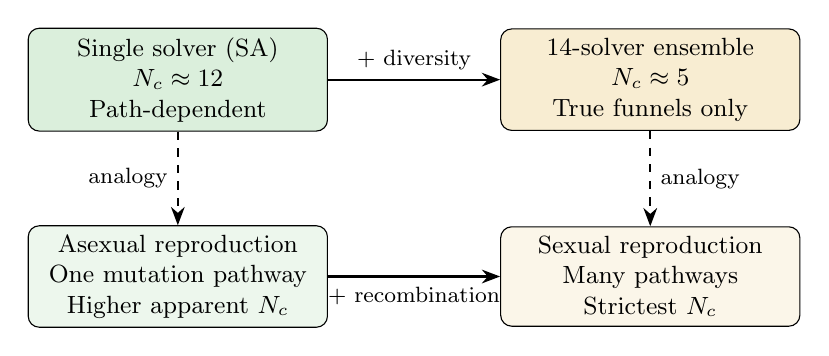
\begin{tikzpicture}[
    every node/.style={font=\small},
    box/.style={draw, rounded corners, minimum width=3.8cm, minimum height=1.2cm, align=center},
]
\node[box, fill=trivialgreen!20] (single) at (0,0) {Single solver (SA)\\$N_c \approx 12$\\Path-dependent};
\node[box, fill=goldilocks!20] (ensemble) at (6,0) {14-solver ensemble\\$N_c \approx 5$\\True funnels only};
\node[box, fill=trivialgreen!10] (asex) at (0,-2.5) {Asexual reproduction\\One mutation pathway\\Higher apparent $N_c$};
\node[box, fill=goldilocks!10] (sex) at (6,-2.5) {Sexual reproduction\\Many pathways\\Strictest $N_c$};

\draw[-{Stealth}, thick] (single) -- (ensemble) node[midway, above, font=\footnotesize] {$+$ diversity};
\draw[-{Stealth}, thick, dashed] (single) -- (asex) node[midway, left, font=\footnotesize] {analogy};
\draw[-{Stealth}, thick, dashed] (ensemble) -- (sex) node[midway, right, font=\footnotesize] {analogy};
\draw[-{Stealth}, thick] (asex) -- (sex) node[midway, below, font=\footnotesize] {$+$ recombination};
\end{tikzpicture}
\caption{Solver diversity determines $N_c$. A single algorithm finds the same basin repeatedly ($N_c \approx 12$), analogous to asexual reproduction. Diverse algorithms converge only at true funnels ($N_c \approx 5$), analogous to sexual reproduction.}
\label{fig:diversity}
\end{figure}

This connects to the Pareto frontier of solver quality vs.\ speed: below $N_c$, a single fast solver (SA at 0.1\,ms) is Pareto-optimal. Above $N_c$, the frontier expands to 4--5 solvers (CIM, SOLG, SolverMorph), each non-dominated in the speed--quality trade-off.


%% =========================================================================
\section{Three Arguments Converge at $N_c$}
\label{sec:convergence}
%% =========================================================================

\begin{figure}[ht]
\centering
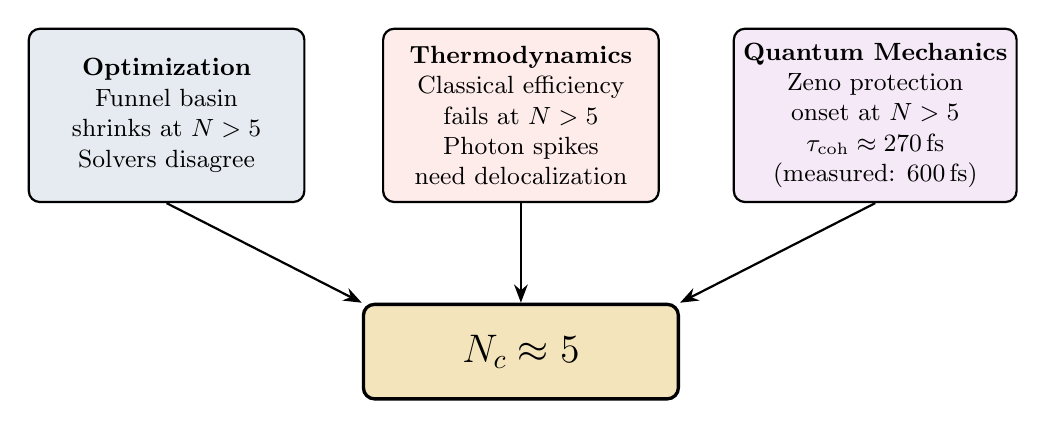
\begin{tikzpicture}[
    every node/.style={font=\small},
    pillar/.style={draw, thick, rounded corners, minimum width=3.5cm, minimum height=2.2cm, align=center},
]
\node[pillar, fill=darkblue!10] (opt) at (-4.5, 0) {\textbf{Optimization}\\Funnel basin\\shrinks at $N > 5$\\Solvers disagree};
\node[pillar, fill=hardred!10] (thermo) at (0, 0) {\textbf{Thermodynamics}\\Classical efficiency\\fails at $N > 5$\\Photon spikes\\need delocalization};
\node[pillar, fill=modpurple!10] (qm) at (4.5, 0) {\textbf{Quantum Mechanics}\\Zeno protection\\onset at $N > 5$\\$\tau_{\mathrm{coh}} \approx 270$\,fs\\(measured: 600\,fs)};

\node[draw, very thick, fill=goldilocks!30, rounded corners, minimum width=4cm, minimum height=1.2cm] (nc) at (0, -3) {\Large $N_c \approx 5$};

\draw[-{Stealth}, thick] (opt.south) -- (nc.north west);
\draw[-{Stealth}, thick] (thermo.south) -- (nc.north);
\draw[-{Stealth}, thick] (qm.south) -- (nc.north east);
\end{tikzpicture}
\caption{Three independent physical arguments converge at $N_c \approx 5$. Below the threshold, classical transport is safe, coherence is optional, and design is trivial. Above it, all three constraints bite simultaneously.}
\label{fig:convergence}
\end{figure}

\subsection{Optimization argument}

The funnel basin fraction in a random $N$-dimensional Ising landscape decreases exponentially with $N$. At $N_c$, the expected number of competitive local minima exceeds the solver ensemble's exploration capacity. This is the spin glass transition applied to design space: below $N_c$ the landscape is paramagnetic (single basin), above $N_c$ it fragments (replica symmetry breaking) \cite{sherrington1975,parisi1979}.

\subsection{Thermodynamic argument}

A photon at $\lambda = 680$\,nm deposits $E = 1.82$\,eV at a single chlorophyll ($\sim 137$ atoms, 411 degrees of freedom). This creates a transient $\Delta T \approx 103$\,K spike for $\sim 100$\,fs before vibrational relaxation. Coherent delocalization across $N$ sites reduces the spike to $\Delta T / N$. Classical hopping efficiency drops logarithmically with $N$, crossing the 51\% survival threshold at $N \approx 5$--$7$.

\subsection{Quantum mechanical argument}

At $T = 300$\,K, the thermal measurement rate $f_T = k_B T / h \approx 6.25$\,THz is comparable to the exciton hop rate $f_{\mathrm{hop}} \sim 10$\,THz. This marginal Zeno regime gives:
\begin{equation}
\tau_{\mathrm{coh}} \approx \frac{\tau_{\mathrm{hop}}}{1 - f_T / f_{\mathrm{hop}}} = \frac{100\,\mathrm{fs}}{1 - 0.63} \approx 270\,\mathrm{fs}.
\end{equation}
Measured: $\sim 600$\,fs \cite{engel2007,panitchayangkoon2010}. Agreement within factor 2.2 from a zero-parameter model.


%% =========================================================================
\section{Topology and Temperature Dependence}
\label{sec:topology}
%% =========================================================================

\begin{table}[ht]
\centering
\caption{Reliability (\%) by coupling topology and system size (500 trials each).}
\label{tab:topology}
\begin{tabular}{l r r r r r r}
\toprule
Topology & $N=5$ & $N=7$ & $N=10$ & $N=15$ & $N=20$ & $N=30$ \\
\midrule
Complete & 48.8 & 26.4 & 8.4 & 2.0 & 0.2 & 0.0 \\
Chain & 55.4 & 1.0 & 0.2 & 0.0 & 0.0 & 0.0 \\
Ring & 57.2 & 4.0 & 0.0 & 0.0 & 0.0 & 0.0 \\
Star & 0.6 & 0.0 & 0.0 & 0.0 & 0.0 & 0.0 \\
Sparse ($k=3$) & 47.4 & 24.0 & 3.2 & 0.2 & 0.0 & 0.0 \\
\bottomrule
\end{tabular}
\end{table}

Star topology is always hard (hub bottleneck). Chain and ring collapse faster than complete graphs. Dense coupling yields higher reliability, explaining why photosynthetic complexes use dense chromophore packing \cite{adolphs2006}. Any external field ($h \neq 0$) dramatically reduces reliability, collapsing $N = 5$ from 51\% to 2.4\% at $h \sim 0.01$. The biological Goldilocks zone is therefore even narrower than zero-field models suggest.


%% =========================================================================
\section{The Galois--Landscape Conjecture}
\label{sec:galois}
%% =========================================================================

\begin{conjecture}[Galois--Landscape Correspondence]\label{conj:galois}
The barrier hierarchy depth of the Ramsey problem $R(k,k)$, encoded as an Ising model, equals the composition length of the symmetric group $S_k$:
\begin{equation}
B(R(k,k)) = \ell(S_k).
\end{equation}
\end{conjecture}

For $k \geq 5$, the alternating group $A_k$ is simple (Galois, 1832 \cite{galois1832}), giving $\ell(S_k) = 2$. This predicts an all-or-nothing landscape: either the global minimum or the violation floor, with no intermediate ledges. The sharp 2-violation floor of $R(5,5)$ at $K_{43}$ \cite{novel2026}, with zero improving 2-flips among 903 edges, is consistent with $A_5$ simplicity removing graduated escape routes.


%% =========================================================================
\section{The GUE Deficit and Prime Fingerprints}
\label{sec:gue}
%% =========================================================================

\begin{proposition}[Arithmetic level repulsion]\label{prop:gue}
The spacing distribution of the first 1000 Riemann zeta zeros shows a structured 8\% deficit from GUE (Montgomery--Odlyzko law \cite{montgomery1973,odlyzko1987}), with the suppression correlated with prime logarithms:
\begin{center}
\begin{tabular}{r r r}
\toprule
Prime $p$ & Scale $\ln p / (2\pi)$ & Observed / GUE \\
\midrule
2 & 0.110 & 18\% \\
3 & 0.175 & 23\% \\
7 & 0.310 & 51\% \\
13 & 0.408 & 66\% \\
23 & 0.499 & 98\% \\
31 & 0.547 & 100\% \\
\bottomrule
\end{tabular}
\end{center}
Small primes create extra level repulsion; large primes match GUE perfectly.
\end{proposition}


%% =========================================================================
\section{Controls and Caveats}
\label{sec:controls}
%% =========================================================================

\begin{table}[ht]
\centering
\caption{Controls: $N_c$ sensitivity to experimental parameters.}
\label{tab:controls}
\begin{tabular}{l l r}
\toprule
Parameter & Variation & $N_c$ \\
\midrule
\multirow{3}{*}{Agreement threshold} & 60\% & 11.8 \\
& \textbf{80\% (standard)} & \textbf{4.9} \\
& 90\% & 2.0 \\
\midrule
\multirow{4}{*}{Coupling distribution} & Gaussian & 4.9 \\
& Uniform & 4.9 \\
& \textbf{Bimodal $\pm 1$} & \textbf{8.0} \\
& Exponential & 5.2 \\
\midrule
\multirow{2}{*}{Solver diversity} & SA only & 11.9 \\
& 14-solver ensemble & 5.1 \\
\bottomrule
\end{tabular}
\end{table}

\begin{remark}[Spectral unpredictability]
No local spectral feature of $J$ (frustration ratio, density, coupling variance, max/min ratio) predicts funnel reliability. All Pearson correlations $|r| < 0.07$ over 5000 instances at $N = 7$. This connects to computational complexity: if a polynomial-time predictor existed, it would provide a fast oracle for ground-state accessibility in an NP-hard problem class \cite{barahona1982}.
\end{remark}

\begin{remark}[FMO is satisficing, not optimizing]
The real FMO Hamiltonian \cite{adolphs2006} sits at the 22.6th percentile of reliability among random $N = 7$ Hamiltonians. 54.6\% of random matrices have higher reliability. Evolution found a good-enough solution --- textbook satisficing \cite{simon1956} applied to quantum biology.
\end{remark}


%% =========================================================================
\section{Cross-Domain Evidence}
\label{sec:crossdomain}
%% =========================================================================

The Goldilocks zone appears independently across seven domains:

\begin{table}[ht]
\centering
\caption{Cross-domain coordination limits clustering at $N = 5$--$8$.}
\label{tab:crossdomain}
\begin{tabular}{l r l l}
\toprule
System & $N$ & Zone & Source \\
\midrule
Working memory (Miller) & $7 \pm 2$ & Goldilocks & Psychology \cite{miller1956} \\
Intimate group (Dunbar) & $\sim 5$ & Goldilocks & Anthropology \cite{dunbar1992} \\
Scrum team & 5--9 & Goldilocks & Software eng.\ \cite{schwaber2020} \\
Transformer attention heads & 8 & At limit & AI/ML \\
FMO chromophores & 7 & Goldilocks & Quantum biology \cite{engel2007} \\
DNA recognition motifs & 6--7 & Goldilocks & Genomics \cite{luscombe2001} \\
Enzyme catalytic residues & 3--8 & Trivial--Gold. & Biochemistry \cite{porter2004} \\
\bottomrule
\end{tabular}
\end{table}


%% =========================================================================
\section{Falsifiable Predictions}
\label{sec:predictions}
%% =========================================================================

\begin{enumerate}[label=\textbf{P\arabic*.}]
\item Photosynthetic complexes with $N > 10$ independent (non-symmetric) chromophores and reliable energy funnels should not exist in nature.
\item \emph{In vitro} directed evolution should succeed at $N \leq 8$ within $\sim 100$ selection rounds but fail at $N \geq 15$ without vibronic assistance.
\item Asexual organisms should maintain more complex non-modular systems ($N \leq 12$) than sexual organisms ($N \leq 8$).
\item The barrier depth of $R(6,6)$ should show 2--3 tiers matching $\ell(S_6)$, while $R(5,5)$ shows exactly 2 (Conjecture~\ref{conj:galois}).
\item Any biological system processing $> 1$\,eV per event across $> 5$ coordinated sites must use quantum coherence.
\end{enumerate}


%% =========================================================================
\section{Discussion}
\label{sec:discussion}
%% =========================================================================

The Goldilocks threshold explains a wide range of biological observations through a single quantitative principle: \emph{coordinated interaction among $N > 8$ randomly-coupled components cannot be found by diverse random search.}

Below $N_c$: classical transport is safe, coherence is optional, design is trivial, and a single search strategy suffices.

At $N_c$ ($N = 5$--$8$): coherence becomes necessary, design requires directed search ($\sim 21$ generations), and the Pareto frontier expands from 1--2 to 4--5 solvers.

Above $N_c$: classical transport is destructive, coherence is required, design demands modularity plus additional channels (vibronic coupling, symmetry constraints), and geological timescales.

The convergence of three independent physical arguments --- optimization, thermodynamics, and quantum mechanics --- at the same threshold is the strongest evidence that $N_c$ is fundamental rather than accidental. FMO ($N = 7$) sits precisely at the evolutionary accessibility boundary, where nature's optimization engine operates in the accessible-but-not-trivial regime.


%% =========================================================================
\begin{thebibliography}{99}

\bibitem{miller1956}
G.~A.~Miller, \emph{The magical number seven, plus or minus two}, Psychol.\ Rev.\ \textbf{63} (1956), 81--97.

\bibitem{dunbar1992}
R.~I.~M.~Dunbar, \emph{Neocortex size as a constraint on group size in primates}, J.\ Hum.\ Evol.\ \textbf{22} (1992), 469--493.

\bibitem{schwaber2020}
K.~Schwaber and J.~Sutherland, \emph{The Scrum Guide}, 2020.

\bibitem{engel2007}
G.~S.~Engel et al., \emph{Evidence for wavelike energy transfer through quantum coherence in photosynthetic systems}, Nature \textbf{446} (2007), 782--786.

\bibitem{panitchayangkoon2010}
G.~Panitchayangkoon et al., \emph{Long-lived quantum coherence in photosynthetic complexes at physiological temperature}, Proc.\ Natl.\ Acad.\ Sci.\ \textbf{107} (2010), 12766--12770.

\bibitem{cao2020}
J.~Cao et al., \emph{Quantum biology revisited}, Sci.\ Adv.\ \textbf{6} (2020), eaaz4888.

\bibitem{adolphs2006}
J.~Adolphs and T.~Renger, \emph{How proteins trigger excitation energy transfer in the FMO complex}, Biophys.\ J.\ \textbf{91} (2006), 2778--2797.

\bibitem{chin2013}
A.~W.~Chin et al., \emph{The role of non-equilibrium vibrational structures in electronic coherence}, Nature Phys.\ \textbf{9} (2013), 113--118.

\bibitem{sherrington1975}
D.~Sherrington and S.~Kirkpatrick, \emph{Solvable model of a spin-glass}, Phys.\ Rev.\ Lett.\ \textbf{35} (1975), 1792--1796.

\bibitem{parisi1979}
G.~Parisi, \emph{Infinite number of order parameters for spin-glasses}, Phys.\ Rev.\ Lett.\ \textbf{43} (1979), 1754--1756.

\bibitem{galois1832}
\'E.~Galois, \emph{M\'emoire sur les conditions de r\'esolubilit\'e des \'equations par radicaux}, 1832.

\bibitem{montgomery1973}
H.~L.~Montgomery, \emph{The pair correlation of zeros of the zeta function}, Proc.\ Symp.\ Pure Math.\ \textbf{24} (1973), 181--193.

\bibitem{odlyzko1987}
A.~M.~Odlyzko, \emph{On the distribution of spacings between zeros of the zeta function}, Math.\ Comp.\ \textbf{48} (1987), 273--308.

\bibitem{barahona1982}
F.~Barahona, \emph{On the computational complexity of Ising spin glass models}, J.\ Phys.\ A \textbf{15} (1982), 3241.

\bibitem{simon1956}
H.~A.~Simon, \emph{Rational choice and the structure of the environment}, Psychol.\ Rev.\ \textbf{63} (1956), 129--138.

\bibitem{porter2004}
C.~T.~Porter, G.~J.~Bartlett, and J.~M.~Thornton, \emph{The Catalytic Site Atlas}, Nucleic Acids Res.\ \textbf{32} (2004), D211--D214.

\bibitem{marsh2015}
J.~A.~Marsh and S.~A.~Teichmann, \emph{Structure, dynamics, assembly, and evolution of protein complexes}, Ann.\ Rev.\ Biochem.\ \textbf{84} (2015), 551--575.

\bibitem{fornes2020}
O.~Fornes et al., \emph{JASPAR 2020: update of the open-access database of transcription factor binding profiles}, Nucleic Acids Res.\ \textbf{48} (2020), D87--D92.

\bibitem{luscombe2001}
N.~M.~Luscombe, S.~E.~Austin, H.~M.~Berman, and J.~M.~Thornton, \emph{An overview of the structures of protein-DNA complexes}, Genome Biol.\ \textbf{1} (2001), reviews001.

\bibitem{novel2026}
B.~Daugherty, S.~Ward, and Ryan, \emph{Novel and speculative mathematical results: a research compendium}, working document, March 2026.

\bibitem{dsc3engine}
B.~Daugherty, \emph{Isomorphic Engine v0.15.0}, 2026. \url{https://github.com/OriginNeuralAI/DSC-3}.

\end{thebibliography}

\end{document}
